\section{Introduction}

Social media platforms contribute to vast amounts of raw and unprocessed data, and advancements in technologies such as machine learning and artificial intelligence have made it possible to transform this data into valuable insights for businesses and researchers alike \cite{sivarajah2017critical}. Australia alone has approximately 21 million social media users \cite{fiber2026social}, while the number of active users worldwide exceeds 3 billion. These platforms provide a rich source of information that can be used to analyse public opinion and identify broader social and political trends.
\\

Social media also plays a significant role in shaping how individuals perceive events, form opinions, and engage with political discourse. In this paper, we investigate public sentiment surrounding the 2025 Australian federal elections and Australian political sentiment by analysing trends in social media discussions. We aim to understand if using text analysis methods we can understand public attitudes before, during and after the elections, and identify significant political events. However, this large influx of social media data requires a scalable and efficient infrastructure for storage, indexing, and querying relevant content. Our solution aims to build such an infrastructure to enable the analysis of political trends data at scale.
\\

In this study, we gathered data from multiple platforms including Bluesky, Mastodon, YouTube and GDELT Project. We focused on text-based data, such as social media posts or video comments. We conducted both emotion detection and sentiment analysis on the texts using open source models in order to enrich the data for analysis. While sentiment analysis broadly categorises text as positive, negative, or neutral, emotion classification captures more nuanced affective states such as anger, fear, joy, sadness, anticipation, and optimism. In the context of political discourse, these distinctions are particularly meaningful: a post may be classified as broadly negative while being primarily driven by fear rather than anger, which carries very different implications for how the public is responding to a candidate or political event. For this reason, our system performs both sentiment and emotion analysis on every harvested post, enabling a richer characterisation of public opinion over time.
\\

The volume and velocity of social media data also introduce significant engineering challenges. Traditional data processing architectures are ill-suited to the continuous, real-time nature of social media streams, where data arrives unpredictably and in varying volumes. To address this, we adopt a cloud-native, event-driven architecture deployed on the Melbourne Research Cloud (MRC), NeCTAR, leveraging Kubernetes for container orchestration, Fission for serverless function execution, and Valkey as a message queue to decouple data ingestion from processing. This architecture allows the system to scale dynamically with data volume and ensures that spikes in social media activity do not result in data loss or processing failures.
\\

The choice of data sources was also guided by the goal of capturing a broad and representative picture of Australian political discourse. Mastodon and Bluesky represent emerging decentralised platforms with growing Australian user bases, while YouTube provides access to comment-level reactions to political content from mainstream media channels. The GDELT Project complements these social media sources by providing structured event data derived from global news coverage, allowing us to correlate social media sentiment with real-world political events reported in the press. Together, these sources offer a multi-platform perspective on public opinion that no single data source could provide alone.

\section{System Architecture Overview}

We will now present an overview of the system architecture we designed and implemented, before going into further detail into the data gathering and processing in the following sections. We will do a deeper dive into overall implications of our architecture at a later section (\ref{TechnicalDiscussion}).

\begin{figure}[H]
	\label{fig:SystemOverview}
	\begin{center}
		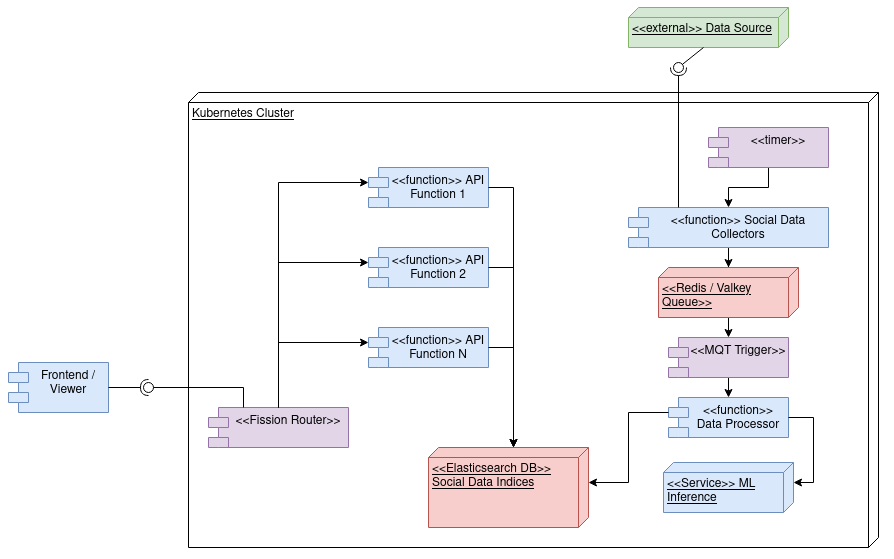
\includegraphics[width=0.75\textwidth]{./assets/ArchitectureOverview.png}
	\end{center}
    \caption{System Architecture Overview.}
\end{figure}

\subsection{Data Ingestion}
This process is handled by a collection of harvester functions deployed on Fission, an open-source Function as a Service (FaaS) framework \cite{fission2026docs} that runs on our Kubernetes cluster. Each data source is assigned to a separate harvester function, which is triggered by a timer setup on Fission. Instead of writing directly to the database, these harvesters publish raw records to a Valkey message queue, decoupling ingestion from processing and allowing the system to deal with sudden spikes in data volume without disrupting and overwhelming the downstream components. This design avoids the traditional Extract-Transform-Load \cite{vassiliadis2009survey} paradigm toward a more event driven approach, which is better suited to the continuous and unpredictable nature of social media data

\subsection{Data Processing}
The processing is implemented as a Fission function triggered by Kubernetes Events-Driven Autoscaling (KEDA), which is suitable for making micro-overscale with respect to the number of events that make the application alive \cite{molleti2022kubernetes}, whenever records are available on the Valkey queue. Each invocation of the processor receives a single raw record, which is then normalised and transformed to map it to a common schema. It then enriches it with machine learning derived features before writing it to Elastic Search. The use of KEDA allows the number of parallel processor instances to scale dynamically with queue depth, ensuring that periods of high ingestion do not result in processing backlogs.

\subsection{Machine Learning Inference}
To enrich the collected social media posts with sentiment scores and emotion classifications, we included a dedicated machine learning inference service deployed as a standalone Kubernetes deployment. This service exposes a simple HTTP API consumed by the processing function and runs two ONNX-optimised transformer models. Open Neural Network Exchange (ONNX) is an open-source format for artificial intelligence models, including both deep learning and traditional machine learning. It defines an extensible computational graph model, operators, and standard data types, which provides a common IR for different frameworks \cite{jin2020compiling}. The first model is a sentiment analysis model trained on social media text, and the second model is a general-purpose sentence embedding model for semantic representation. Deploying this as a persistent service rather than a fission function was a deliberate decision due to the startup latency associated with loading transformer models into memory. This would have been prohibitive in a short lived serverless context. The service is stateless and can be horizontally scaled by increasing the number of replicas in its deployment configuration.


\subsection{Storage and Analytics}
The processed and enriched records are stored in ElasticSearch. ElasticSearch serves as both the primary data source and the analytics engine. Its document-oriented approach makes it able to efficiently search information, where schema-less data, in the form of arbitrarily complex JSON documents, can be handed to Elasticsearch for indexing \cite{elasticsearch2018software}. We maintain two categories of indices - provider-specific indices that preserve the raw schema of each data source for validation and source-level exploration, and a common unified index that normalises records from all providers under a single schema to enable cross-platform comparison. ElasticSearch’s native support for full-text search, aggregations and vector similarity search makes it well suited to the range of analytical queries . It handled weekly sentiment aggregations and keyword-based topic filtering.


\subsection{API and Frontend}

Data is surfaced to end users through a Flask-based HTTP API, which exposes endpoints for querying sentiment trends, emotion distributions, candidate and party data, and census information. The API accepts topic names and associated keywords and returns pre-aggregated weekly time series data drawn from ElasticSearch. The API is implemented as Fission functions which query the ElasticSearch Database and can be called by the frontend to display analytics. The frontend itself is implemented as a Streamlit application. It uses an HTTP client to interact with our functions via the Fission router and HTTP triggers and thus pull aggregated data from ElasticSearch.
